\chapter{rs-fMRIs and Patient Motion}
\label{ch:mri}

This chapter discusses rs-fMRIs and how they are affected by patient motion. Specific topics include the structure of rs-fMRIs, sources of motion, quantifying motion, and a review of current methods for preventing and managing motion in rs-fMRIs.

\section{Structure of an rs-fMRI}

rs-fMRIs are discrete representations of continuous data. A new image volume of the patient's brain is acquired every two to three seconds. The image volume is composed of a three-dimensional version of a pixel called a voxel (volume element). Just as the ``distance'' between each image volume encompasses a certain amount of time, each voxel encompasses a small volume of physical space. The transformations between the continuous physical and temporal dimensions and the discrete physical and temporal dimensions are the spatial and temporal resolutions. 
The concept of a 4D rs-fMR image is illustrated in two different ways in Figure \ref{ch2:fig:rsfmri-views}. The first representation is an ordered list of 3D image volumes where each voxel contains a single numeric value. The second representation is a single 3D image volume, where the value of each voxel is a temporal signal.

An rs-fMRI is considered to have a relatively low spatial resolution but high temporal resolution. The physical size of a single voxel seems small at about 4 mm$^3$, but this resolution is not granular enough to capture details about activity within small structures of the brain. The activity information recorded during an rs-fMRI must be combined with the detailed anatomic information from a structural MRI to know precisely which areas of the brain are active at each point in time. A structural MRI volume takes much longer to acquire than an rs-fMRI volume, which can be obtained every two to three seconds. Unfortunately, the patient's position and neural activity can change faster than the image volume can be acquired. As a result, a temporal resolution of two to three seconds is not fast enough to actively compensate for sources of noise which confound the BOLD signal. 

\begin{figure}
\centering
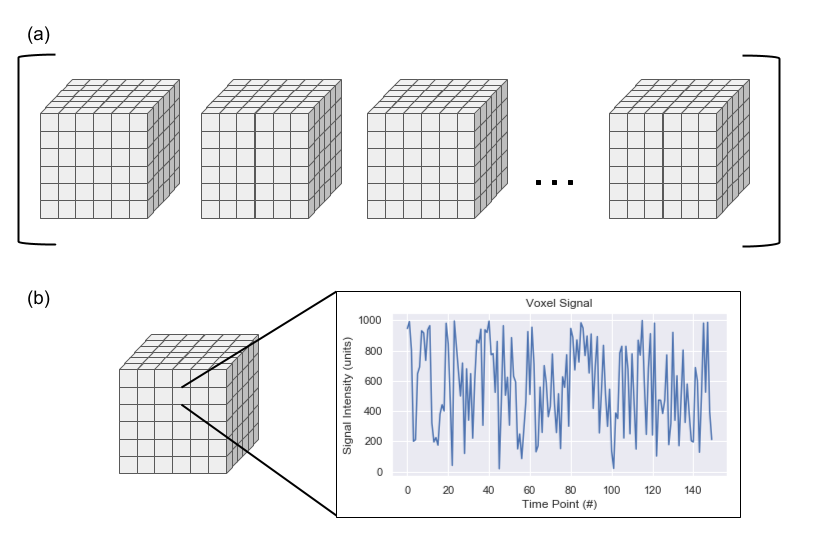
\includegraphics[width=.75\textwidth]{2/rsfMRI-views.png}
\caption{A rs-fMRI can be thought of (a) as a sequence of image volumes or (b) as a single volume where each voxel contains a temporal signal rather than a single numeric value.}
\label{ch2:fig:rsfmri-views}
\end{figure}

\clearpage

\section{Factors Impacting rs-fMRIs}

The BOLD signal present inside a patient's brain is not recorded with complete accuracy by an MRI scanner. Even if the same patient exhibited precisely the same BOLD signal during two different scans, the recorded image sequences would vary slightly. Several factors impact the image sequence viewed by a radiologist, and we give an overview of them in Figure \ref{ch2:fig:signal-filters}. 

The first factor in Figure \ref{ch2:fig:signal-filters} is the patient's physiology. An rs-fMRI is not sensitive enough to detect brain activity on a neuronal level. Instead, it measures the changes in the amounts of deoxygenated hemoglobin in the brain. The deoxygenated hemoglobin quantities are highly correlated with brain activity because active areas of the brain use more oxygen than inactive areas, but the BOLD signal is still only an approximation of brain activity.

The second factor in Figure \ref{ch2:fig:signal-filters} represents the changes to the signal that occur due to patient motion.
During every medical imaging scan, the patient will naturally perform small, automatic movements due to regular bodily functions. Minuscule movements caused by cardiac activity may disrupt scans with high spatial resolution or with high sensitivity to the movement of blood molecules. More significant movements caused by respiration result in motion artifacts in images of the thoracic and abdominal cavities. 

\begin{figure}
\centering
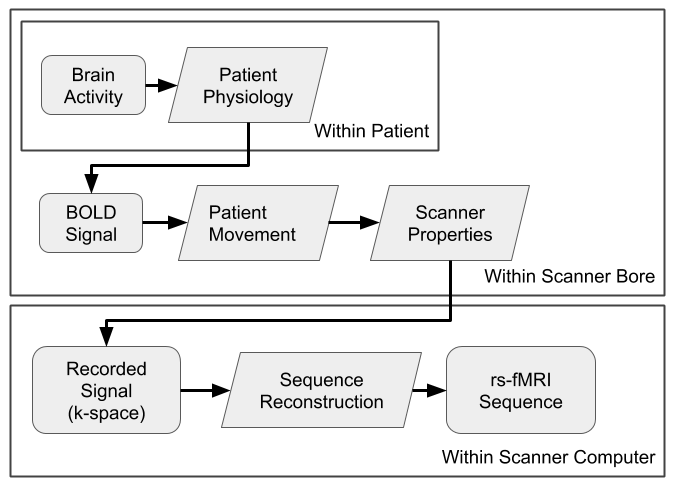
\includegraphics[width=.6\textwidth]{2/rsfMRI-signal-filters.png}
\caption{The patient's brain activity is affected by several factors before an MRI scanner produces a visually interpretable image sequence. (The rounded rectangles represent the signal at different stages of recording while the rhombuses represent the primary factors.)}
\label{ch2:fig:signal-filters}
\end{figure}

Other motions occur on a larger and more conscious scale. It is important to note that different populations may exhibit more of certain macro-motions than others. The patient may fidget or shift his gaze when he becomes bored in the scanner. If the patient falls asleep during a scan, there may be slight movement as the body relaxes and re-tenses if the patient wakes. Certain MRI protocols are known to produce loud sounds: during one of these protocols, the patient may become surprised and react by jumping. Additionally, claustrophobic patients or patients who feel secure around specific people that are not allowed in the scanner room may become agitated. 

Both the small-scale, automatic motions and the large-scale, reflexive motions corrupt the BOLD signal. These effects of patient motion will be discussed in-depth in the next~section.

The third factor in Figure \ref{ch2:fig:signal-filters} is the unique properties of the scanner. The acquired image sequence will vary slightly even in machines made by the same company because each scanner has a unique primary magnetic field, $B_0$. The $B_0$ inhomogeneities can be measured using a primary field map. These field maps can be used to correct signals displaced by the $B_0$ field, though they cannot be used to recover signals corrupted by the field.

The final factor is also related to the properties of the MRI scanner. The image sequence produced by a scanner is dependent on the scanner vendor. Different vendors use different proprietary algorithms to convert the signal recorded by the scanner in k-space into a visually interpretable image sequence. Between the $B_0$ inhomogeneities and the scanner vendor differences, the differences in the scanners used to acquire the sequences must be resolved before images from different scanners can be compared.

\section{Effects of Patient Motion}

Due to their low spatial and high temporal resolutions, rs-fMRIs are highly susceptible to all types of motion outlined in the previous section. In general, motion affects an acquired image sequence in three ways. The first and most obvious effect is the position of the patient changes throughout the sequence. The second effect is due to the way changes in the patient's position affect the signal recorded by the scanner. The third effect is related to the magnetic fields in patient tissue and changes in their orientation within $B_0$. These three effects will hereafter be referred to as the positional effect, the spin history effect, and the susceptibility effect of motion.

\subsection{The Positional Effects of Motion}

The technique used for analyzing neuronal network activity rs-fMRIs, called functional connectivity analysis, assumes that the contents of one voxel at every time point during the sequence all contain signals from a single point in the brain. This assumption is vital in the process of inferring networks of neuronal activity. 

While rs-fMRIs have a spatial resolution on the order of millimeters, neuronal activity occurs on the spatial resolution of microns. As a result, each voxel in an rs-fMRI volume contains information from a number of neurons. The smallest movement of the patient can alter the voxel to which a cluster of neurons contributes. These seemingly insignificant changes can alter the position of the patient enough to cause the voxels to record signals from different brain regions or even tissue types. This change in voxel location within the brain violates the assumption that single voxels record from the same location within the brain for the duration of the sequence.

\subsection{The Spin History Effects of Motion}

In addition to changing the recorded position of the patient, motion impacts the established spin gradients, which introduces artifacts into the image sequence.

During an ideal MRI scan, the patient is sitting in the scanner and all molecules become aligned with the primary magnetic field $B_0$ in a relaxed state. Then, a radiofrequency (RF) pulse is applied to the field. The purpose of the pulse is to excite the molecules in a particular volume of physical space change their orientation to match the induced perpendicular field. When the pulse ends, the molecules precess back to their orientation in $B_0$. As they do, their small magnetic fields induce electric currents on the RF coil. The currents are recorded by the scanner as signals in frequency space. The volume of the space intended to be excited is known, and the signal produced by the induced electric current is used in conjunction to reconstruct the image in voxel space.

However, when the patient moves, the volume of space which was thought to be excited is not actually excited: some other volume of space, which may or may not overlap with the intended volume of space, is excited instead. Because the MRI scanner has no way to know this assumption is not correct, it does not know that not all of the molecules in its intended area are relaxed and correctly aligned to the $B_0$ field at the end of the RF pulse. The scanner proceeds with the next RF pulse, which excites a new set of ``relaxed molecules'', some of which are still excited from the previous pulse. As a result, the signals produced in the second RF pulse are different than they should be. Signals that are artificially decreased result in dark shadows within motion affected volumes of the sequence, while signals that are artificially increased result in bright spots.

The previous few paragraphs in this section describe how motion disrupts the magnetic spin gradients present in the patient during an rs-fMRI scan. The spin gradients need time to recover to the correct magnetic field orientation, and up to eight to ten seconds may pass before the recovery is complete \cite{Power2014}. While the spin gradients are reorienting, the recorded BOLD signal will vary more than expected between temporally neighboring volumes. These variations are more difficult to quantify than the positional effects of motion.

The nature of the $B_0$ field in an MRI scanner can be recorded using a field map. Acquiring a field map while the patient is in the scanner records information about how the patient interacts with the $B_0$ field. These field maps of the patient in the scanner can be used to perform distortion correction on the acquired sequence. A study of the effects of distortion correction on rs-fMRIs of 40 healthy subjects suggested that distortion correction using field maps can increase the functional connectivity in rs-fMRIs \cite{Togo2017}.

\subsection{The Susceptibility Effects of Motion}

The susceptibility of a material describes how the material will behave when placed in a magnetic field. Most materials are either paramagnetic or diamagnetic. Paramagnetic materials are attracted to and align with magnetic fields. Diamagnetic have the opposite interaction: they are repelled from and become anti-aligned with magnetic fields. Additionally, paramagnetic materials contribute to the magnetic field, while diamagnetic materials detract from it. 

Both types of materials cause distortions in the magnetic field. These distortions are prominent in stronger magnetic fields and at the interface of two different material types. In MRI scanners, the differences in susceptibility between soft tissue and bone or between soft tissue and air can produce artifacts in the acquired sequence. These artifacts are amplified when the patient moves. When the patient moves, the interfaces between tissues and air distort the $B_0$ field. The distortions in the $B_0$ field change the electromagnetic signal recorded by the scanner and lead to spurious correlations during the analysis of the rs-fMRI sequence.

Susceptibility artifacts can be reduced using susceptibility maps. Susceptibility maps are short acquisitions that use multiple echo periods to detect small changes in the location of susceptibility interfaces in an MRI sequence. They are not part of most rs-fRMI acquisition protocols.

\section{Measuring Motion}

Even though we described three effects of motion on rs-fMRIs in the previous section, these effects impact the sequence in two areas: the position of the patient and spurious signal correlations throughout the sequence.

\subsection{Measuring Motion: Patient Position} 

The effect of motion on patient position is measured as the difference in the positions of subsequent image volumes. The difference in position is determined using metrics calculated by performing rigid volume registration on the two volumes. 
In rigid volume registration, one volume is chosen as the reference volume and the other is the moving volume. The reference volume remains stationary while the moving volume is translated and rotated in three-dimensional space on top of it. The registration is complete when the position of the patient in the moving volume matches the position in the reference volume. 

The moving volume can undergo linear or nonlinear transformations. Linear transformations include translation, rotation, and affine transformations along all three spatial dimensions as well as a scaling transformation. These transformations move the image volume as a whole: all voxels in the moving image remain in the same location relative to their neighbors. On the other hand, nonlinear transformations can warp the contents of the moving volume so that it better matches the contents of the reference volume. Nonlinear transformations are more complex than linear transformation. They involve additional image processing steps such as smoothing and voxel interpolation.

\begin{figure}
\centering
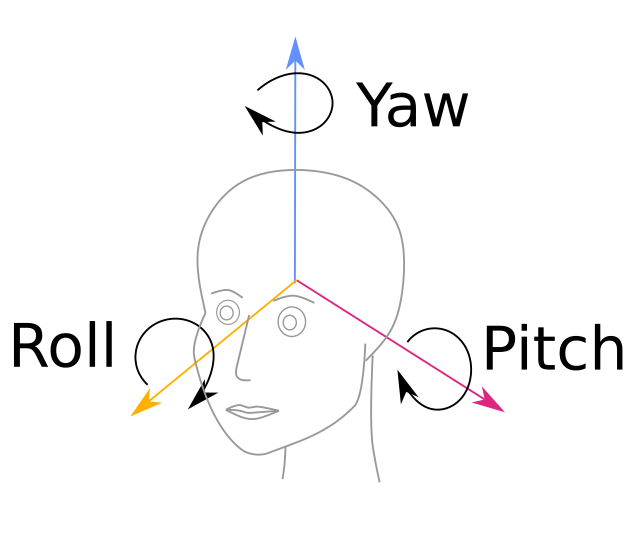
\includegraphics[width=.6\textwidth]{2/pitch_roll_yaw.png}
\caption{The pitch, roll, and yaw rotations describe rotations or an object about three orthogonal axes whose origin is in the object's center of mass.}
\label{fig:pry}
\end{figure} 

Even in cases when nonlinear transformations are used, the registration process begins with the translation and rotation transformations. The three translation and three rotation parameters used to achieve the best alignment are used to calculate the positional change between the image volumes. The positional change between temporally neighboring volumes is called the framewise displacement (FD).  

Several researchers have proposed slightly different methods for calculating the FD. Power et al., Jenkinson et al., and Dosenbach et al. each propose a slightly different method for calculating the FD \cite{Power2012} \cite{Jenkinson2002} \cite{Dosenbach2017}. All three FD calculations produce correlated metrics: the FD metric proposed by Power et al. produces measurements approximately twice as large as the metric proposed by Jenkinson et al., and Dosenbach et al. reported a high correlation between their FD and Power’s FD \cite{Yan2013a} \cite{Dosenbach2017}. 

In the remainder of this document, the abbreviation FD refers to Power et al.'s version of the FD metric, which is calculated as:

\begin{equation}
FD(J_i) = | \Delta d_{ix} | + | \Delta d_{iy} | + | \Delta d_{iz} | \\ + | \Delta \alpha_i | + | \Delta \beta_i | + | \Delta \gamma_i |
\end{equation}

\noindent where $J_i$ is the image volume $i$, $| \Delta d_{i *} |$ are the magnitude of change in position along the $x$, $y$, and $z$ axes between volumes $i$ and $i-1$, and $| \Delta \alpha_i |$, $| \Delta \beta_i |$, and $| \Delta \gamma_i |$ are the magnitude of change in pitch, roll, and yaw between volumes $i$ and $i-1$, respectively. A diagram outlining how pitch, roll, and yaw relate to the human head can be seen in Figure \ref{fig:pry}.

\subsection{Measuring Motion: Spurious Signal Correlations}

Both the spin history and susceptibility effects of motion contribute to alterations in the signal recorded and reconstructed by the MRI scanner. Without $B_0$ field maps and susceptibility maps, it is difficult to separate the impact of each of these factors on the recorded signal. We assume at this point that both the spin history and the susceptibility effects contribute equally to changes in the recorded signal intensity.

One popular metric to measure changes in the recorded signal due to patient motion was developed by Smyser et al. in 2010. Their metric is called DVARS, which measures the temporal \textbf{d}erivative of the root mean squared \textbf{var}iance over the voxels between two volumes \cite{Smyser2010}. Power et al. explain the steps to calculate DVARS in a separate study \cite{Power2012}. The DVARS value is calculated in two steps. The first step uses backward differences to approximate the derivative of the BOLD signal change between volumes $J_i$ and $J_{i-1}$ at every point $\vec{x}$ contained in both image volumes:

\begin{equation}
\frac{\partial}{\partial t} J_i(\vec{x}) \approx J_i(\vec{x}) - J_{i-1}(\vec{x}).
\end{equation}

The second step calculates the root mean square of the approximated derivatives for all $N$ points $\vec{x}$:

\begin{equation}
DVARS(J_i) = \sqrt{ \frac{1}{N} \sum_{\vec{x} \in J_i, J_{i-1}} \left( \frac{\partial}{\partial t} J_i(\vec{x}) \right)^2 }.
\end{equation}

DVARs measures the change in BOLD signal intensity, which is highly related to motion-induced spin gradient changes. 

\subsection{Acceptable Motion Quantities}

Even though the effects of motion on the patient position and the recorded signal can be measured, we still need gold standard criteria to determine whether an image containing motion can be used. Patients move slightly due to breathing and cardiac function, and the BOLD signal naturally fluctuates over time. Some motion is expected; however, we need to know how much motion can be present in the image before it is considered to be corrupted by it. Power et al. established thresholds for FD and DVARS to determine the usability of a pair of images:
\begin{itemize}
\item FD less than or equal to 0.2 mm from the previous volume, and
\item DVARS less than or equal to 25 units on a normalized scale of [0, 1000] signal units \cite{Power2014}
\end{itemize}

\noindent Image volumes that meet these criteria are considered to be low-motion.

The minimum duration of low-motion data is highly debated. van Dijk et al. established that approximately five minutes of low-motion data is sufficient for use in functional connectivity analysis \cite{VanDijk2012}. However, a recent study by Laumann et al. suggests that at least 10 minutes of low-motion data is essential for obtaining high-quality results \cite{Laumann2015}. From a practical standpoint, it is difficult to obtain even five minutes of low motion data from certain patient populations, so radiology technicians and neuroimaging study designers are often content with the five minute time standard. 

\section{Motion Prevention}

During an MRI scan, thick foam pads of various sizes and shapes are used to isolate and immobilize the area of interest on the patient. While these pads impede most motion, especially in compliant patients, additional techniques and protocols are often used to prevent patients from moving during the image acquisition process. Not all of these techniques are suitable for all patient populations, and some techniques have been designed specifically for certain populations.

\subsection{Pre-Scan: Education}

Educational material can be used to help the patient understand what to expect during an MRI scan as well as to teach the patient different behavioral coping strategies. The education materials can be used either before or upon arrival at the imaging facility. Most of the formal literature focuses on informative, distraction, and behavioral techniques to use during pediatric MRI scans, though many of the following approaches could be adapted for use with adults.

In a review of the available literature, Alexander found several commonly used techniques to educate pediatric patients before and comfort or distract pediatric patients during radiology procedures \cite{Alexander2012}. Tools such as educational coloring books and short videos can expose patients to the types of equipment they can expect to see using a familiar, engaging medium. Pediatric patients can learn coping strategies to employ during the scan, such as breathing techniques, imagery, and positive statements. Alexander notes that allowing a pediatric patient to choose a behavioral coping strategy gives the patient a sense of control and may encourage the patient to cooperate during the MRI acquisition.

Mock scanners and MRI simulators can also help the patient feel more comfortable during the scan. Barnea-Goraly et al. showed that both a commercial MRI simulator and a low-tech mock scanner desensitized pediatric patients between four and ten years of age to the MRI scanner with the results that 92.3\% of the acquired images could be used in high-resolution anatomical studies \cite{Barnea-Goraly2014}. 

% distraction
Several groups have investigated the role of auditory and visual distraction during an MRI acquisition. Headphones with music and stories or MR compatible video goggles can distract patients from the tedium of the scan \cite{Alexander2012} \cite{Barnea-Goraly2014} \cite{Harned2001}. Khan et al. found that a relatively simple moving light show can help distract younger patients \cite{Khan2007}. Garcia-Palacios et al. performed a case study comparing the efficacy of music and immersive virtual reality tools as distractions during a mock scan \cite{Garcia-Palacios2007}. They suggest that immersive virtual reality may help decrease patient anxiety during a scan more effectively than music alone. As virtual reality technology improves, it may join headphones and MR compatible video goggles as an available distraction method.

Another valuable source of distraction for pediatric patients could be the patient's parent or parents. Having a parent involved with the scanning process may calm the patient and encourage him to cooperate; however, parental distress can further upset an anxious patient and complicate the scanning process \cite{Alexander2012}. 

These techniques for educating the patient and helping the patient cope with the anxiety that can accompany an MRI scan all depend on the ability of the patient to understand instructions and communicate with the scan team. Due to the gap in communication abilities, these techniques are not useful for young patients such as neonates, infants, toddlers, and possibly elementary school-aged children. Other patient populations, such as those with developmental delays and neurobehavioral disorders, may also have difficulty adhering to these protocols. Even in patients with developed and intact communication skills, the techniques outlined here do not actively prevent the patient from moving during the scan: they only help the patient feel more comfortable with the MRI environment.

\subsection{During Scan: Sedation}

Sedation can be used to help a patient tolerate an MRI scan. Murphy and Brunberg retrospectively analyzed seven weeks of data from the MR department and found that 14.2\% of their adult patients required some form of sedation \cite{Murphy1997}. In a study about claustrophobia and MR acquisitions, Dewey et al. report that out of 55,734 patients who underwent MRI scans, a total of 1004 patients experienced claustrophobia, and 610 of these patients required intravenous sedation before their scans \cite{Dewey2007}. Even though sedation allowed the patients mentioned in this paragraph to undergo an MRI scan, the authors of both studies note that sedation can result in adverse events and advise the reader to avoid patient sedation if possible.

Sedation can be used with pediatric patients, though the risks are more significant than with adult patients. Studies have shown that sedation for pediatric imaging can lead to hypoxemia and inappropriate sedation levels during image acquisition \cite{Malviya2000}. Pediatric patients can also expect ``motor imbalance and gastrointestinal effects,'' as well as agitation and restlessness for several hours after waking from sedation.

A report from the American Academy of Pediatrics and the American Academy of Pediatric Dentistry outlines the minimum set of criteria needed for a pediatric patient to be sedated for a procedure \cite{Cote2016}:
\begin{itemize}
\item The patient must be a suitable candidate for sedation based on their medical history and medical needs.
\item The patient's health status must be evaluated and verified by the sedation team before the procedure.
\item Informed consent must be obtained before the procedure.
\item Instructions for what to expect and how to transport the patient home safely must be provided to the patient's responsible adult.
\item At least one responsible adult must be with the patient at the medical facility. Furthermore, the report recommends that two adults are present for patients who travel to and from the facility using car seats. This practice ensures that one adult can monitor the patient after the procedure while the other adult drives.
\item The patient's food and drink intake before the procedure should be taken into account to minimize the risk of pulmonary aspiration.
\item The clinician administering the sedation must have immediate access to emergency facilities, personnel, and equipment and should monitor the patient for adverse events, including respiratory events, seizures, vomiting, and allergic reactions.
\item There must be a clear protocol outlined for immediately accessing these emergency services.
\item Emergency equipment and drugs appropriate for the patient's size and age must be immediately available in case the patient needs to be resuscitated.
\item The information about the procedure must be correctly documented.
\item The facility should have a dedicated recovery area, and the status of the patient should be recorded when he is discharged. The patient should not be discharged if his levels of consciousness and oxygen saturation do not meet recognized guidelines.
\item The patient may be held at the facility for prolonged monitoring after the procedure.
\end{itemize}
\noindent This report clearly states that the levels of monitoring suggested above should serve as minimum levels of involvement: clinicians should increase patient monitoring as needed for complex cases. Rutman has a similar and detailed perspective on patient monitoring during and after sedation, adding that two independent medical personnel should be present during the scan, and one of them should be present until the patient is discharged \cite{Rutman2009}. Rutman also notes that all sedation and monitoring equipment must be MR compatible, which is a simple but important safety constraint. This constraint makes sedation less advisable if the appropriate equipment is not available.

Sedation in neonatal and infant populations is not recommended. The  U.~S.~Food and Drug Administration (FDA) issued a warning in late 2016 about repeated use of sedation or general anesthesia for patients under three years of age or pregnant women during their third trimester \cite{FDA2016}. The warning states that while a single, relatively short exposure to sedative and anesthetic drugs is unlikely to impact the patient, the effects of prolonged exposure to these drugs are still being studied. Studies of sedative and anesthetic drugs in multiple animal models have shown that these drugs can lead to loss of nerve cells in the brain when the animals undergo prolonged, repeated exposure to them during this period of brain development. More data is needed to determine if this effect translates to humans.

\subsection{During Scan: Feed and Sleep Protocols}

Neither sedation nor educational and behavioral techniques are appropriate to use with neonatal patients, but rs-fMRIs in neonates and infants are invaluable in studying early brain development and neurological diseases \cite{Smyser2015}. A set of protocols has been developed specifically for scanning neonates without sedation. These protocols are referred to as ``feed and sleep'' or ``feed and bundle'' protocols.

Windram et al. describe a protocol in which the infant is deprived of food for four hours before the scan \cite{Windram2011}. At the scanning facility, the patient is fed by his mother, swaddled, and placed in a vacuum-bag immobilizer for the duration of the scan. 

Rather than deprive the patient of food before the scan, Gale et al.'s protocol recommends timing the scan so that the patient is fed after arrival on-site and less than 45 minutes before the scan \cite{Gale2013}. The patient's ears are protected from the noise of the MR scanner by a layer of dental putty followed by headphones and held in place by a hat. The patient is then swaddled and placed in the scanner once he is asleep. Additional foam padding is used to cushion the patient's head and provides extra noise protection.

Mathur et al. describe a protocol similar to the previous two: the patient's feeding schedule is adjusted so that he feeds 30-45 minutes before the scan time, and he is swaddled, given ear protection, and placed in a vacuum-bag immobilizer \cite{Mathur2008}.

When performed correctly, these protocols are generally successful, and the neonatal patient will sleep for the duration of the MRI scan. However, the patient may shift slightly while asleep or may wake up and move mid-scan.


\section{Prospective Motion Correction}

Since motion cannot be completely eliminated from rs-fMRI scans, different approaches have developed for correcting for the effects of motion after the scan. These approaches can be divided into two groups: those that monitor the patient's motion during the scan and those that work solely on the acquired sequences.

\subsection{Optical Motion Correction}

Several groups have developed methods for actively accounting for changes in the patient's position during an MRI scan. Optical-based methods record the patient's position using a combination of markers placed on the patient, and one or more MR compatible optical cameras placed the scanner bore. The changes in the patient position from one timepoint to the next are used to update the MR parameters in real-time. Real-time updates of the MR parameters result in decreased spatial and spin-history effects of motion in the acquired sequences.

The first report of successful prospective motion correction using optical cameras and markers was by Zaitsev et al. in 2006 \cite{Zaitsev2006}. Their dual-camera system was located outside of the MRI scanner and focused on the patient inside the system. Four reflective markers were attached to a modified mouthpiece initially designed for patient immobilization. Changes in the translation and rotation of the patient were recorded and processed during the exam. The processed changes were sent in real-time to the MRI scanner, which used them to update the gradient orientations, RF frequencies, and RF phases at every time point during the acquisition process.

Aksoy et al. simplify this approach by using a single in-bore optical camera and replacing the 3D markers with a small 2D chessboard grid \cite{Aksoy2008}. Intrinsic camera properties, as well as information about the camera's placement within the MRI scanner, were recorded prior to the scan as part of a calibration process. During the scan, patient movements recorded using the optical camera were used to calculate the relationship between the patient's position at the current time point in the physical space and the patient's position at the initial time point in the MR space. The transformation needed to translate between these two positions was calculated on a laptop and passed to the MRI scanner to correct for motion in real-time. The camera used to record the position of the chessboard is mounted on the head coil. If the patient moves his head significantly, the camera will only be able to record the position of part of the chessboard marker. This limitation makes it difficult for the computer vision processing to identify the independent features on the standard chessboard. 

Forman et al. modified the chessboard marker to improve its use for high-motion patients \cite{Forman2011}. To differentiate between the different blocks in the chessboard, they added a unique, machine-readable symbol to each black block in the chessboard. The symbols were chosen to be unique even in the event of rotation so that the identification of each block would be robust to rotation movements. The chessboard marker was embedded with MR-detectable agar so that the position of the marker could be detected in the MRI scan as well as by the in-bore camera. At each point during the scan, the image recorded by the in-bore camera was sent to a computer independent from the MRI controller. The independent computer detected the blocks of the chessboard and identified their spatial locations using the symbols contained within them. Their positions were checked by confirming the locations of the symbols with respect to each other. The confirmed locations of the corners of the black boxes were used to estimate the position of the patient, which was then sent to the MRI controller so that the magnetic gradients and RF hardware could be updated for the time point. The authors note that the latency of the system is a significant limitation to their system, but overall they experienced an increase in the accuracy of the estimates of the patient's position.

Several companies have developed commercial products for prospective motion correction in neurological images. KintetiCor's system uses a high-resolution camera and a physical marker to detect motion \cite{kineticor}. The camera's resolution allows it to detect respiratory and cardiac motion through changes in skin displacement on the patient's forehead. The physical marker consists of a pair of rectangles containing several concentric circles that are connected via a bridge across the nose. Any patient movement is reflected in the movement of the markers, which is also tracked through the camera. Both the camera system and the marker are MR compatible. Another company, TracInnovations, uses a stereo camera system to track all patient motion \cite{tracinnovations}. At the start of the scan, the stereo camera obtains a point cloud (a set of single point coordinates in space) specifying the patient's position at that time. The points in the point cloud are averaged together to create a primary marker. Small facial motions, cardiac motion, and respiratory motion are monitored using the point cloud. Larger head motions are monitored using both the point cloud and the primary marker. These two systems both allow prospective motion correction to be turned on or off. If the prospective motion correction is off, the system will still acquire the motion parameters so that the motion can be corrected retrospectively.

The methods and technologies discussed above have a few limitations due to the optical camera setups. For precise real-time motion correction, the camera or cameras must be carefully placed so that the position of the marker on the patient can be recorded. They must have a clear line of sight, which means they will be in the same room as the MRI scanner, if not within the scanner bore. The cameras and markers must be MR compatible, and the positions of the cameras and markers in physical space relative to the visual markers on the patient must be known. These positions are vital for the calculations used to measure the motions. Even if the motion measurements are accurate, the changes in position that are recorded and used to adapt the scan parameters will only be valid for rigid body motion of the body part to which the markers are attached: any distortion of soft tissue will not be accurately accounted for during the motion correction unless the camera system was explicitly built for and trained to do so. 

Systems using markers attached to patient suffer from these limitations, but also from limitations due to the markers themselves. If the marker is not attached correctly to the patient, the marker can slip and move independently from the patient. The whole purpose of the markers is that they provide a known set of visual features that can be used to determine how a patient moved because they moved with the subject.

\subsection{Non-Visual External Sensors}

Cameras are not the only type of external sensor that can be used to measure motion during an rs-fMRI scan. 

There is a class of sensors that can take advantage of the electrophysical properties of an MRI scanner. These sensors include wired nuclear magnetic resonance field probes, wireless inductivity coupled markers, and off-resonance markers. %CITATIONS AND DETAILS. 
The fact that these sensors directly interact with the magnetic field of the MR scanner means that protocols using these sensors must be modified to account for them. As a result of the protocol modification, the scan time might need to be extended.

As mentioned earlier in this chapter, respiration and cardiac activity are sources of patient motion. The most straightforward way to reduce the effect of respiratory motion is to instruct the patient to hold their breath at specific intervals during the scan. One alternative to breath-holding uses the periodic nature of respiration. Since respiration is relatively periodic, it can be monitored and accounted for within a scan protocol via gating. A comparative study of breath-holding and respiratory gating in MRIs of the coronary arteries suggests that images acquired using respiratory gating had 76\% better quality than the images acquired using breath-holding \cite{PMID:7822549}.

In cases where only respiration is taken into account, gating prevents an image from being acquired unless the patient is in the specified state. In the case of respiration, the specified state is either complete inhalation or exhalation. The state of a patient's respiration can be tracked using respiration bellows. After acquiring the MRI sequence, volumes in the sequence can be grouped depending on when they were recorded in the breathing cycle. By only using volumes recorded during the same stage of the breathing cycle, the effects of respiratory motion can be mitigated. This approach to gating will increase the amount of scanner time needed.

When both cardiac and respiratory motions are considered, the patient's respiration is monitored through a bellows or pressure belt, and their cardiac activity is monitored on a delay during the scan through a pulse oximeter on the patient's finger \cite{Hu1995}. The cardiac and respiratory data are synchronized with the acquired image after the scan. The synchronized signals are then used to remove changes in the image associated with physiological motion, which ``substantially reduces image-to-image fluctuations'' \cite{Hu1995}.

For macro-scale motions, electromagnetically sensitive trackers can be placed on the patient and used to monitor changes in position during the scan. Afacan et al. used a tracker produced by Robin Medical Inc. (Baltimore, MD) to measure the position and orientation of subjects relative to the center of the scanner bore \cite{Afacan2016}. The tracker consisted of two sensors that were attached to the patient's forehead. The sensors recorded their $x$, $y$, and $z$ coordinates as well as two vectors indicating their orientations at every magnetic activation. These measurements were processed and displayed for a technician in real-time during each scan.

Ultimately, using external sensors to monitor the patient for inherent physiological motion can improve the quality of the obtained MR images. However, the addition of extra sensors complicates the process and set up of rs-fMRI scans.

\subsection{Image Signal Motion Monitoring}

Dosenbach et al. have developed a tool to evaluate motion in rs-fMRI sequences as they are acquired \cite{Dosenbach2017}. It registers each volume to the initial volume of the rs-fMRI sequence immediately after the new volume is recorded. The parameters produced by this registration are used to calculate the framewise displacement between pairs of volumes, which is then compared to a set of displacement thresholds associated with the scan quality. The number of volumes that meet each threshold is used to determine how many more volumes are needed to obtain five minutes of low motion volumes. This method for assessing the quality of a scan in real-time is useful for ensuring images are acquired with a sufficient number of low-motion volumes. It can also aid the technologists in determining whether to prematurely terminate a scan, which may be desirable if the amount of time needed to obtain enough low motion volumes is greater than the amount of time remaining for the patient in the scanner. 


\subsection{General Limitations of Prospective Motion Correction}

All types of prospective motion correction introduce a delay into the scanning process. The delay is due to the additional processing of some metrics to determine the patient's position, the transmission of these metrics to the MR scanner, and the adjustments the scanner makes to its next set of measurements. These alterations to the image acquisition during prospective motion correction actively change the image as it is acquired.
Maclaren et al. note that while prospective motion correction reduces inhomogeneities in the $B_0$ field, the $B_0$ field will still change when the patient moves and may change while the motion correction is occurring \cite{Maclaren2013}. % SO WHAT?

In order to view a scan not impacted by prospective motion correction, the patient often must undergo a second scan. It may be wise to build the second image acquisition into the same scan period as the prospectively motion-corrected scan: unsuccessful prospective motion correction has the potential to drastically corrupt the acquired scan \cite{Zaitsev2017}.

Finally, though prospective motion correction has great power for managing motion during a scan, it cannot be used to recover motion-corrupted data in existing data sets.


\section{Retrospective Motion Correction}

Many groups have put significant effort into developing techniques for motion correction after the scan is acquired. Here, we discuss several commonly used techniques: volume registration, denoising, and filtering.

\subsection{Volume Registration}

The rs-fMR image is stored in computer memory as a set of 3D matrices. The values in corresponding cells of each matrix are considered to be aligned in this digital space (voxel space). The voxel space is defined by the imaging protocol and relates to the physical space through the spatial resolution of the image. Even though the spatial and voxel spaces for the image align, the contents of the image volumes may be misaligned due to patient movement. Because we cannot assume that an image is entirely motion-free, we cannot directly compare the contents of each image volume in the rs-fMRI sequence. However, we can use image registration to align the contents of the image volumes to reduce the impact of motion on patient position.

Image registration is the process of morphing the contents of one image so that they overlap optimally with another image. The morphing operations include translation, rotation, scaling, skewing, and nonlinear adjustments. The linear and affine operations in this list should be used to perform rigid body registrations for organs such as the brain. Nonlinear operations can be used to fine-tune the alignment of more pliable organs such as the liver. All morphing operations are applied to one image repeatedly until it is contents optimally match those of the static reference image as determined by a chosen similarity metric. 

One of the earliest examples of image registration was described by Friston et al. in 1995 \cite{Friston1995}. They performed image registration on positron emission tomography (PET) scans and MRI scans of a human brain. During the registration process, one scan was designated as the ``reference'' image, which remained stationary, and the other scan was designated as the ``object'' image, which was transformed to match the reference image. Constraining the alignment process to transform a single image into the coordinates of the other image rather than transforming both images into an independent coordinate frame simplifies the registration process.

\begin{figure}
\centering

\includegraphics[width=.7\textwidth]{2/traditional-registration.png}
\caption{The traditional approach to volume registration in an rs-fMRI sequence consists of registering all volumes in the sequence to a single reference volume.}
\label{fig:ch4:traditional-reg}
\end{figure}

When performing image registration on a sequence of image volumes, one volume must be chosen as the reference volume for the entire sequence. All other volumes in the sequence are registered to this volume. An example of this process can be seen in Figure \ref{fig:ch4:traditional-reg}. In subsequent work, Friston et al. used the first volume in the rs-fMRI sequence as the universal reference image \cite{Friston1996}. Common choices for the reference volume include the volume with the least positional difference to all other volumes in the sequence, a volume produced by averaging all volumes in the sequence, or the first volume in the sequence \cite{Friston1996} \cite{Liao2005}. In our implementation, we chose to use the first volume in the sequence as the reference volume.

One drawback to this traditional approach to volume registration is that it only minimizes the differences between all the image volumes in the sequence and the reference volume. The keyword here is ``minimizes'': minimizing differences between image volumes does not mean that there are no differences between the image volumes. Image registration is an optimization problem, and its goal is to find the overlap between a pair of volumes with as few differences as possible either within a defined number of iterations or until the optimization cost does not change above a certain tolerance for a certain amount of time. These practical constraints on optimization problems mean that there may still be differences between other pairs of image volumes in the sequence that do not include the reference volume. 

Variations on Friston et al.'s framework have been developed over the last two decades. Liao et al. suggested that an rs-fMRI sequence could be viewed as a hidden Markov model, and reflected this idea in their suggested registration framework \cite{Liao2016}. They still use the first volume in the image sequence as the reference volume. Their framework uses the transformation of the previous volume to the reference volume to initialize the transformation for the current volume and the reference volume. 

It has been demonstrated that image registration across the entire image sequence reduces the effects of motion on the image sequence, though they do note that motion also affects the image due to changes in the spin history of the image. These effects are not correctable by global volume registration alone and will be discussed later in this chapter.

\subsection{Denoising}

Denoising techniques can be applied to an rs-fMRI after global volume registration is completed. They consist of regressions of various confounding variables. 

It is relatively common for researchers to use rigid realignment parameters calculated during volume registration as signals to remove via regression. The realignment parameters are the translations along and the rotations about the $x$, $y$, and $z$ axes \cite{Power2012}. These six parameters and their first-order derivatives are suggested as regression parameters by several researchers \cite{Power2012} \cite{Satterthwaite2012} \cite{VanDijk2012}. 

While the realignment parameters and their derivative for the current image volumes help reduce the effects of motion on an image sequence, these parameters are not sufficient on their own. As the effects of motion on rs-fMRIs have been studied, it has been established that motion at one point in the sequence can affect the next several volumes. Researchers have decided to address this effect by incorporating the rigid realignment parameters from surrounding timepoints into the regression parameters for any given current image volume \cite{Power2014} \cite{Satterthwaite2013} \cite{Yan2013a}.

Patriat et al. performed a robust comparison of different regression parameters on their MotSim motion data set \cite{Patriat2017}. They included rigid realignment parameters, but also used parameters obtained by performing principal component analysis (PCA) on the image sequences. PCA generates a set of linear, uncorrelated components that reflect the main features of a patient's motion. The list of parameter combinations included 
\begin{itemize}
\item 12mot: The six rigid realignment parameters and their first derivatives,
\item 12for: The first 12 principal components of the whole brain before realignment,
\item 12back: The first 12 principal components of the whole brain after realignment,
\item 12both: The first 12 principal components of the whole brain both before and after realignment,
\item 24mot: the six rigid realignment parameters of the current volume, the six rigid realignment parameters of the previous volume, and the square of these rigid realignment parameters,
\item 24both: the first 24 principal components of the whole brain before and after realignment.
\end{itemize}

\noindent They found that the features extracted from the image sequence using PCA explained more variance in the image sequence (measured using $R^2$) than the rigid realignment parameters. They showed that increasing the number of regressors increased the amount of variance explained, but with diminishing returns. While their work is promising, their experiment was performed on a simulated data set using healthy subject data and required an accurate estimate of the subject's head motion.

In addition to the positional effects of motion, the spin history and susceptibility effects of motion must be considered. Signals associated with these effects are called nuisance signals. One common nuisance signal is the global signal of the image sequence. Global signal regression (GSR) corrects for variance between temporal signals within a voxel and for the mean BOLD signal across all voxels \cite{Power2014} \cite{Satterthwaite2013} \cite{Yan2013} \cite{Yan2013a}. GSR has been shown to reduce spuriously increased long-distance correlations in functional connectivity studies, but may inadvertently weaken shorter-distance connections \cite{Jo2013} \cite{Power2014}  \cite{Satterthwaite2012}. Other nuisance signals that can be removed via regression are signals white matter and cerebral spinal fluid (CSF) \cite{Power2014} \cite{Satterthwaite2013}. The impact of removing these signals from the image sequence is limited: in some cases, removing white matter and CSF signals do not reduce the effects of motion on the BOLD signal \cite{Yan2013a} \cite{Jo2010}.

Another set of signals that may be removed via regression are components identified using techniques such as principal component analysis (PCA) or independent component analysis (ICA) \cite{Pruim2015} \cite{Salimi-Khorshidi2014} \cite{Behzadi2007}. Though both PCA and ICA decompose a set of data into a list of signals, the properties of the lists are different. PCA produces a list of orthogonal signals that best represent the features of a data set ordered from most representative to least representative. ICA treats the problem of decomposing the image sequence into different source signals as a blind source separation problem. ICA separates components by maximizing their statistical independence but requires additional help to identify the correct number of components. The set of components produced by ICA are assumed to be independent, non-Gaussian, and less complex than the original signal. For more details about ICA, refer to Section \ref{section:ica}. Regression of each of these sets of signals has been shown to reduce the effects of motion in the sequence, but neither removes them entirely \cite{Power2015} \cite{Parkes2017}. 

\subsection{Filtering}

Not all patients move in the same ways or at the same rate. In some cases, a patient will perform a large and sudden movement and then settle into a position close to their original position. The volumes containing the motion can be removed from the rs-fMRI sequence to create smaller, motion-free sequences. Several studies have found that subsequences of data of the same patient can be concatenated to produce a single, longer sequence without impacting the functional connectivity analysis. The process of detecting and removing motion-corrupted volumes has been formalized into several filtering techniques. 
Three popular filtering techniques are scrubbing, spike regression, and despiking. 

\textbf{Scrubbing} begins by examining the image sequence for ``high-motion'' image volumes \cite{Power2012}. Here, ``high-motion'' is defined as image volumes that have 0.5 mm FD and 0.5\% DVARS difference from their preceding volume. The volumes containing at least this quantity of motion, the preceding volume, and two subsequent volumes, are removed from the sequence, resulting in a set of discontinuous subsequences. The discontinuous subsequences can be combined without negatively impacting the functional connectivity analysis of the BOLD signal \cite{Fair2007} \cite{VanDijk2010}. As long as the reconnected subsequences compose a sequence at least 125 frames (approximately 5 minutes) in length, the scrubbed sequence can be used for analysis \cite{Power2012}. Many techniques for temporally filtering high-motion rs-fMRIs have been developed,  though all of them result in the loss of image volumes \cite{Barnes2011} \cite{Fransson2007} \cite{Jones2010} \cite{Kennedy2008} \cite{Smyser2010} \cite{Smyser2011}.  

\textbf{Spike regression} also identifies volumes containing large quantities of motion, though it treats them differently than scrubbing does. \cite{Satterthwaite2013}. It identifies spikes in the image sequence and replaces frames affected by the spikes with interpolated volumes.

A spike is defined as a frame in the sequence where the FD or the FD and the DVARS between it and its previous frame surpass a given set of thresholds. The value of the thresholds greatly impacts the cleaned image sequence. A low threshold will identify more spikes and produce a cleaner image sequence but remove more data, while a high threshold will retain more data but contain more motion artifacts. The thresholds used by Satterthwaite et al. on their adolescent data set are 0.25 mm FD and 1.4\% signal units of DVARS. 

After identifying the spikes in an image sequence, they are modeled as signals to remove through regression. The simplest model of a spike is as a motion event at a single time point. However, it has been established that patient motion may affect several frames in the image sequence. Satterthwaite et al. examined six combinations of frames around the frame in which the spike was based during their analysis of spike regression. They found that removing spikes identified using just the FD threshold and modeled as only effecting a single frame resulted in the fewest different neural connections in the highest and lowest motion images as well as the lowest correlation between functional connectivity and patient motion \cite{Satterthwaite2013}.

\textbf{Despiking} is different from these techniques. It treats the image sequence as a single image volume where each voxel contains an intensity signal. Each intensity signal is examined for sudden changes or spikes. The value of each detected spike is replaced with an interpolated value calculated using the preceding and subsequent points in the voxel's signal \cite{Jo2013} \cite{Patel2014}. Despiking does not remove volumes, but could accidentally remove valuable signals if they appear as outliers in the image voxel signals.

\subsection{Spin History Distortion Correction}

Many post-acquisition methods have been developed specifically to correct for distortions due to the impact of motion on the magnetic field. The usability of these dynamic distortion correction methods has been studied in a few specific cases, but their generalizability has yet to be confirmed in a broader range of fMRI studies \cite{Zaitsev2017}.

\section{Summary}

Resting-state fMRIs are four-dimensional images that record the BOLD signal in active areas of the brain. The BOLD signal can be used to evaluate the functional connectivity of different underlying networks in a patient's brain. Since rs-fMRIs are highly sensitive to motion, clinicians and psychologists have devised techniques to inform patients about what they can expect during an MRI scan as well as different coping mechanisms to help them remain calm during the scan. These techniques do not prevent the patient from moving, but approaches that do are not always appropriate to use during an rs-fMRI scan. Techniques and algorithms to prospectively and retrospectively remove motion from rs-fMRIs have also been developed, though they are not always successful in removing the effects of motion. Ultimately, the amount of motion present in the rs-fMRI sequence dictates whether or not the sequence can be used in clinical or research applications.